\documentclass[conference]{IEEEtran}
\IEEEoverridecommandlockouts
% The preceding line is only needed to identify funding in the first footnote. If that is unneeded, please comment it out.
\usepackage{cite}
\usepackage{amsmath,amssymb,amsfonts}
\usepackage{algorithmic}
\usepackage{graphicx}
\usepackage{textcomp}
\usepackage{xcolor}
\usepackage{float}
\def\BibTeX{{\rm B\kern-.05em{\sc i\kern-.025em b}\kern-.08em
    T\kern-.1667em\lower.7ex\hbox{E}\kern-.125emX}}
\begin{document}


\title{Aprendizagem Supervisionada com RapidMiner e Python: Reconhecimento de atividade em pessoas idosas (Tema C3/ Grupo 31)}

\author{\IEEEauthorblockN{André Lopes dos Santos (200505634)}
\IEEEauthorblockA{\textit{Departamento de Engenharia Informática} \\
\textit{Faculdade de Engenharia da Universidade do Porto}\\
Porto, Portugal \\
up200505634@fe.up.pt}
\and
\IEEEauthorblockN{Bernardo Oliveira Teixeira Santos (201504711)}
\IEEEauthorblockA{\textit{Departamento de Engenharia Informática} \\
\textit{Faculdade de Engenharia da Universidade do Porto}\\
Porto, Portugal \\
up201504711@fe.up.pt}
\and
\IEEEauthorblockN{Miguel Rossi  Seabra (200604224)}
\IEEEauthorblockA{\textit{Departamento de Engenharia Informática} \\
\textit{Faculdade de Engenharia da Universidade do Porto}\\
Porto, Portugal \\
ei06054@fe.up.pt}
}


\maketitle

\begin{abstract}
Aprendizagem supervisionada e seus algoritmos, que são uma componente importante da inteligência artificial. Neste estudo, os algoritmos são usados num determinado conjunto de dados sobre o movimento de idosos com vários sensores. Os algoritmos permitem criar um modelo que nos permite determinar qual a atividade que um idoso está a realizar através dos valores dos sensores.
\end{abstract}

\begin{IEEEkeywords}
Inteligência Artificial, Aprendizagem Supervisionada, Python, RapidMiner
\end{IEEEkeywords}

\section{Introdução}
Neste trabalho utilizar-se-ão diversos métodos de aprendizagem supervisionada para o reconhecimento de atividade em pessoas idosas. 
Para  realizar este estudo, foram implementados diversos algoritmos de aprendizagem supervisionada em RapidMiner (K-Nearest Neighbour, Redes Neuronais e Support Vector Machines) assim como um algoritmo de redes neuronais implementado em Python.

Começar-se-á por mencionar alguns trabalhos relacionados já com estes dados. Posteriormente é explicado o trabalho desenvolvido e quais os parâmetro utilizados nos diferentes testes.

No final mostram-se e explicam-se os resultados obtidos, tirando conclusões dos mesmos.


\section{Trabalho Relacionado}
Existem vários estudos \cite{b1} \cite{b2} \cite{b3} \cite{b4}, com várias abordagens que utilizam inteligência artificial por forma a classificar atividades humanas em tempo real.
Um dos estudos \cite{b1} centra-se na classificação da saída da cama do paciente. Os algoritmos utilizados centram-se na modelação de uma sequência de primeira ordem “Markov Chain”.
Num outro estudo \cite{b2} o objetivo era classificar a saída e da cadeira pelo paciente em tempo real. Este baseia-se na modelação probabilística de sequencias lineares “conditional random fields” (CRF).
À semelhança do estudo referido anteriormente \cite{b2}, um outro estudo \cite{b3} também utilizou CRFs mas utilizando técnicas de “sliding window”.
O algoritmo CRF é igualmente utilizado num outro estudo. \cite{b4}


\section{Trabalho Desenvolvido}

\subsection{Dados Fornecidos}
Os dados utilizados neste estudo, foram recolhidos de um repositório de Machine Learning \cite{b5}, que tem muitos conjuntos de dados já prontos para se poderem realizar este tipo de estudos. Este repositório tem a vantagem de ter dados muito "limpos" (i.e. sem dados em falta, etc.) comparativamente ao que se encontra em situações reais, pelo que será muito mais simples realizar o pré-processamento dos mesmos.

Os dados estão divididos em 9 colunas sendo cada uma o seguinte (citando da fonte):
\begin{itemize}
	\item Column 1: Time in seconds;
	\item Column 2: Acceleration reading in G for frontal axis;
	\item Column 3: Acceleration reading in G for vertical axis;
	\item Column 4: Acceleration reading in G for lateral axis;
	\item Column 5: Id of antenna reading sensor;
	\item Column 6: Received signal strength indicator (RSSI);
	\item Column 7: Phase;
	\item Column 8: Frequency;
	\item Column 9: Label of activity, 1: sit on bed, 2: sit on chair, 3: lying, 4: ambulating; 
\end{itemize}

Os dados em si são anónimos, mas cada ficheiro corresponde a uma pessoa diferente, e a última letra do nome do ficheiro corresponderá ao sexo da pessoa em questão, i.e. "d1p33F", como termina com a letra "F", quer dizer que é uma pessoa do sexo feminino.

\subsection{RapidMiner}
Com o RapidMiner, começou-se por extrair os dados dos diferentes ficheiros, criando duas colunas extras nos dados: uma primeira para identificar a pessoa (através do nome de ficheiro) e a segunda para dizer o sexo da pessoa (extraindo da última letra do nome do ficheiro).

Posteriormente juntaram-se esses dados numa só tabela. Nessa mesma tabela foram retirados algumas colunas que foram consideradas irrelevantes, mais especificamente: Coluna 1: Tempo e Coluna 5: ID da Antena.

Foi escolhido um atributo para servir de "label", que em RapidMiner significa a componente chave que queremos que a aprendizagem consiga prever. No final terá como propósito, através dos outros dados, conseguir prever qual a atividade que uma pessoa está a realizar com base nos outros dados.

Foram Realizados 3 algoritmos de aprendizagem supervisionada: Redes Neuronais, K-Nearest Neighbor e Support Vector Machines. Para cada um deles, foi realizado o método de "Cross-Validation" em que se usaram 5 partições disjuntas (para tornar o procedimento não muito demorado). Na Figura \ref{fig:rapidminer1} pode-se ver uma imagem do "Project" concebido.

\begin{figure}[H]
	\centering
	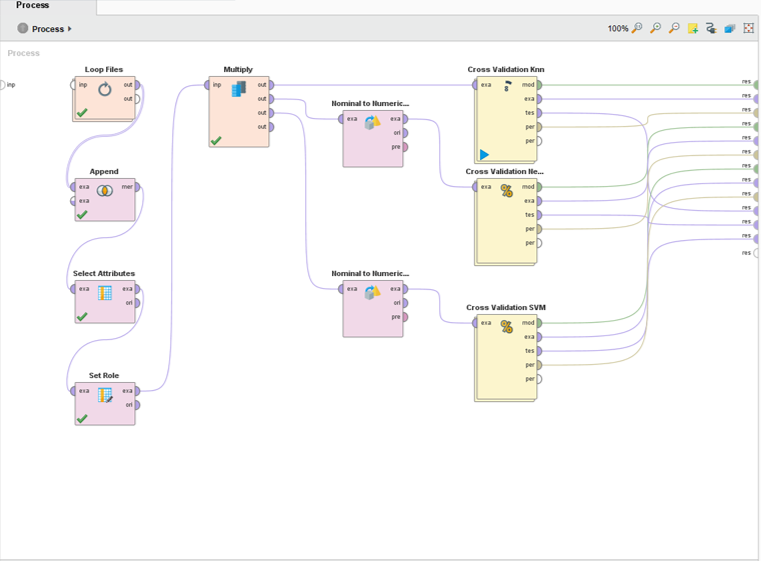
\includegraphics[width=1\linewidth]{Rapidminer1.png}
	\caption{Esquema do Projeto RapidMiner Utilizado.}
	\label{fig:rapidminer1}
\end{figure}

Para os diferentes métodos os parâmetros foram os seguinte:
\begin{itemize}
	\item Para o Método "K-Nearest Neighbor";
	\begin{itemize}
		\item K = 5;
	\end{itemize}
	\item Para o Método "Support Vector Machines"
	\begin{itemize}
		\item Parâmetro C = 0;
		\item Função Kernel: K(x,y) = x*y;
		\item Epsilon de convergência: 0,001
	\end{itemize}
	\item Para as Redes Neuronais:
	\begin{itemize}
		\item Número de ciclos de treino: 200;
		\item "Learning Rate" (peso adicionado): 0.3;
	\end{itemize}
\end{itemize}

Há que enfatizar o facto de que estas Redes Neuronais é do género "Feed-Forward" treinado por um algoritmo de "back propagation" (multi-layer perceptron).


\subsection{Rede Neuronal em Python}
O programa a desenvolvido foi baseado numa implementação encontrada de uma rede neuronal em python \cite{b6}.

Para representar uma Rede Neuronal Artificial em python, foi criada uma classe "Neural\_Network" que tem como atributos o número de nós de entrada na input layer ("n\_inputs"), o número de nós na hidden layer ("hidden\_nodes"), o peso dos nós de entrada ("weight\_input") e o peso dos nós da camada intermédia ("weight\_hnodes").  Esta classe tem os seguintes métodos: a função de ativação para obter o output, representada pela função sigmóide ("sigmoid"), que recebe como argumento um valor ou conjunto de valores; a derivada da função de ativação ("sigmoidPrime") , que recebe como argumento um valor ou conjunto de valores; a função de propagação direta ("forward"), que recebe a matriz de inputs, multiplica-a pelos pesos respetivos, aplica-lhe a função de ativação, multiplica desta vez pelos pesos dos nós intermédios e, por fim, aplica de novo a função de ativação a este último conjunto de valores de forma a obter o output; tem também a função de propagação reversa ("backward"), que recebe a matriz  de inputs, os outputs reais os outputs previstos, calculando as diferenças entre os dois conjuntos de outputs e atualizando os pesos dos nós consoante a magnitude dos erros cometidos; e por fim, a classe tem o método de treino ("train") que recebe os inputs e os outputs reais, aplica a função de propagação direta aos inputs e posteriormente aplica a função de propagação reversa com os inputs , os outputs reais e os valores calculados anteriormente correspondentes ao output previsto.

O programa, após ler e processar os dados de um ficheiro, cria uma nova rede neuronal através da classe criada ("Neural\_Network()") e separa os dados em dados de treino, com os quais vai treinar a rede neuronal, e dados de teste, com os quais vai testar a precisão com que a rede treinada consegue prever os resultados. 

No final, é apresentada uma lista de valores reais comparados com o seu valor previsto pela rede neuronal, além do erro associado a estes cálculos.


\section{Resultados Obtidos}
\subsection{Resultados RapidMiner}


\subsection{Resultados da Rede Neuronal em Python}

Utilizado a Rede Neuronal Desenvolvida em Python, obtiveram-se os seguintes resultados sendo que as "Losses" são basicamente o erro entre o output esperado e o valor real.

\begin{table}[htbp]
\caption{"Training Loss vs Testing Loss" em função do número de iterações}
\begin{center}
\begin{tabular}{|c|c|c|}
\hline
\textbf{Iterações} & \textbf{Training Loss} & \textbf{Testing Loss} \\
\hline
 10000 & 0.14255 & 0.02555\\
 50000 & 0.11119 & 0.02145\\
 100000 & 0.09601 & 0.01953\\
 200000 & 0.08662 & 0.01867\\
 500000 & 0.07341 & 0.01222\\
 1000000 & 0.05612 & 0.00868\\
\hline


\end{tabular}
\label{tab1}
\end{center}
\end{table}


\begin{figure}[H]
	\centering
	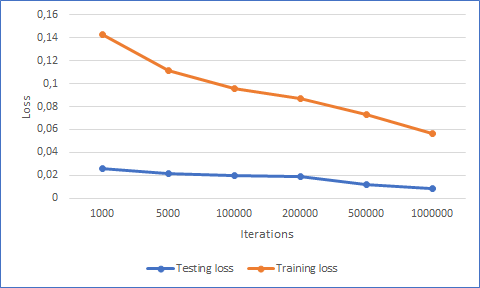
\includegraphics[width=1\linewidth]{python1.png}
	\caption{"Training Loss vs Testing Loss" em função do número de iterações}
	\label{fig:python1}
\end{figure}


O erro nas previsões dos treinos vai decrescendo mais rapidamente do que nas previsões dos testes à medida que se vão aumentando as iterações.
Isto acontece pois o algoritmo é melhorado com os treinos, devido à atualização dos pesos dos nós.

Mesmo assim, as perdas nos treinos obviamente continuam a ser maiores que nos testes, pois as previsões de output para os testes já utilizam um algoritmo bastante treinado



\section{Conclusões}

Através da implementação e aplicação dos diversos algoritmos de Aprendizagem Supervisionada e dos dados fornecidos \cite{b5}, torna-se possível prever, através dos dados dos sensores, qual a atividade que uma dada pessoa está a realizar.

No caso do algoritmo desenvolvido em python, pode-se verificar que quanto maior for o número de iterações, menor serão os "losses", mostrando assim que o algoritmo aprende mais e consegue ser mais preciso nas suas previsões.


\section*{Referencias}


\begin{thebibliography}{00}
\bibitem{b1} A. Wickramasinghe, D. C. Ranasinghe, C. Fumeaux e K. D. Hill, “Sequence Learning with Passive RFID Sensors for Real-Time Bed-Egress Recognition,” IEEE Journal of Biomedical and Health Informatics, pp. 917-929, July 2017.
\bibitem{b2} R. L. S. Torres, R. Visvanathan, S. Hoskins, A. van den Hengel e D. C. Ranasinghe, “Effectiveness of a Batteryless and Wireless Wearable Sensor System for Identifying Bed and Chair Exits in Healthy Older People,” Sensors, nº 16, p. 546, 2016. 
\bibitem{b3}R. L. S. Torres, D. C. Ranasinghe e Q. Shi, “Evaluation of Wearable Sensor Tag Data Segmentation Approaches for Real Time Activity Classification in Elderly,” MOBIQUITOUS 2013, LNICST 131, pp. 384-395, 2014. 
\bibitem{b4} L. S. R. Torres, D. C. Ranasinghe, Q. Shi e A. P. Sample, “Sensor Enabled Wearable RFID Technology for Mitigating the Risk of Falls Near Beds,” em IEEE International Conference on RFID, 2013. 
\bibitem{b5} “UCI Machine Learning Repository: Activity recognition with healthy older people using a batteryless wearable sensor Data Set,” [Online]. Available: http://archive.ics.uci.edu/ml/datasets/Activity+recognition+with+heal\-thy+older+people+using+a+batteryless+wearable+sensor. [Acedido em Maio 2019].
\bibitem{b6} "Build a Neural Network in Python | Enlight" [Online]. Available https://enlight.nyc/projects/neural-network/ [Acedido em Maio 2019]








\end{thebibliography}

\end{document}
